% Stitch-policy intuition guide — v4 streaming LocalAgreement-2
% Source of truth: apps/api/app/services/stream_policy.py + docs/v4/protocol.md §7.
% Build: pdflatex main.tex  (twice for refs)
\documentclass[11pt]{article}
\usepackage[margin=1in]{geometry}
\usepackage{tikz}
\usetikzlibrary{decorations.pathreplacing, patterns, arrows.meta}
\usepackage[T1]{fontenc}
\usepackage{parskip}
\usepackage[hidelinks]{hyperref}

\title{Voice Scribe v4 --- The Stitch Policy, by Intuition\\
\large Every tuning parameter of \texttt{stream\_policy.py}: the failure without it,
and what the tuned value buys}
\author{}
\date{2026-08-05 (policy as of the post-review resolution pass; C7.14 + C9.3 included)}

% ---------- shared visual language ----------
\tikzset{
  word/.style={draw, minimum height=13pt, inner xsep=3pt, inner ysep=2pt,
               font=\scriptsize\ttfamily, anchor=west},
  committed/.style={word, fill=black!75, text=white, draw=black},
  tentative/.style={word, fill=black!6, draw=black!45, text=black!60, densely dashed},
  bad/.style={word, fill=red!65, text=white, draw=red!70!black},
  dup/.style={word, fill=orange!75, text=white, draw=orange!80!black},
  frontier/.style={very thick, red!55!black},
  axis/.style={->, thick},
  lbl/.style={font=\scriptsize, anchor=west},
  rowlbl/.style={font=\scriptsize\bfseries, anchor=east},
  note/.style={font=\scriptsize\itshape, text=black!55, anchor=west},
  win/.style={decorate, decoration={brace, mirror, amplitude=4pt}, thick, black!60},
}

\newcommand{\panelrow}[1]{\node[rowlbl] at (-0.2,0.25) {#1};}

\begin{document}
\maketitle

\noindent
\textbf{Legend.}\;
\tikz[baseline=-2pt]{\node[committed]{word};}\; committed (permanent)\quad
\tikz[baseline=-2pt]{\node[tentative]{word};}\; tentative (may still change)\quad
\tikz[baseline=-2pt]{\node[bad]{word};}\; wrong text\quad
\tikz[baseline=-2pt]{\node[dup]{word};}\; duplicate\quad
\tikz[baseline=-2pt]{\draw[frontier] (0,-0.12) -- (0,0.28);}\; commit frontier

\section*{0. The engine}

Every 750\,ms tick the server re-decodes one window: 3\,s of already-committed
context plus all uncommitted audio. The policy compares this hypothesis with the
previous tick's and commits the longest \emph{agreeing prefix} (case- and
punctuation-insensitive). Everything else stays tentative. Structural rule
(C5.5): every word either commits or withholds --- \emph{none revises}. That is
why ``zero retractions'' is a property of the construction, not a hope.

\begin{center}
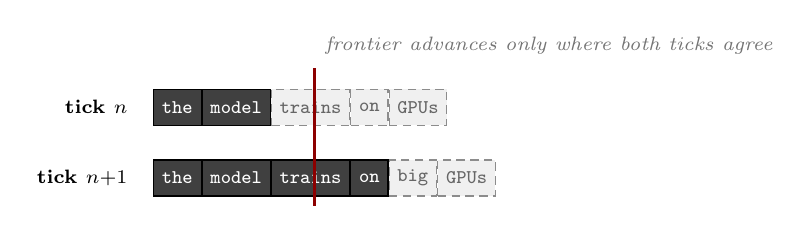
\begin{tikzpicture}[x=1cm]
  \panelrow{tick $n$}
  \node[committed] (a1) at (0,0.25) {the};
  \node[committed, anchor=west] at (a1.east) (a2) {model};
  \node[tentative, anchor=west] at (a2.east) (a3) {trains};
  \node[tentative, anchor=west] at (a3.east) (a4) {on};
  \node[tentative, anchor=west] at (a4.east) (a5) {GPUs};
  \begin{scope}[yshift=-0.9cm]
  \panelrow{tick $n{+}1$}
  \node[committed] (b1) at (0,0.25) {the};
  \node[committed, anchor=west] at (b1.east) (b2) {model};
  \node[committed, anchor=west] at (b2.east) (b3) {trains};
  \node[committed, anchor=west] at (b3.east) (b4) {on};
  \node[tentative, anchor=west] at (b4.east) (b5) {big};
  \node[tentative, anchor=west] at (b5.east) (b6) {GPUs};
  \end{scope}
  \draw[frontier] (2.05,-1.0) -- (2.05,0.75)
     node[note, anchor=south west, yshift=1pt] {frontier advances only where both ticks agree};
\end{tikzpicture}
\end{center}

\noindent The hypotheses agreed on \texttt{trains on}; those commit. The tail
(\texttt{big GPUs} vs \texttt{GPUs}) disagrees; it waits. Ten knobs bound this
loop. Each figure below shows the degenerate setting first --- the failure the
knob exists to prevent --- then the tuned behavior.

\section*{1. \texttt{left\_context\_s = 3.0} --- the decoder never starts cold}

\textbf{Without:} the window opens exactly at the frontier; the model decodes
mid-phrase with no conditioning and mangles the first words.
\textbf{With:} 3\,s of committed audio is re-decoded for conditioning only;
\texttt{localize()} drops the copies \emph{by timestamp}, never by string match
(string matching fails exactly when the model re-punctuates).

\begin{center}
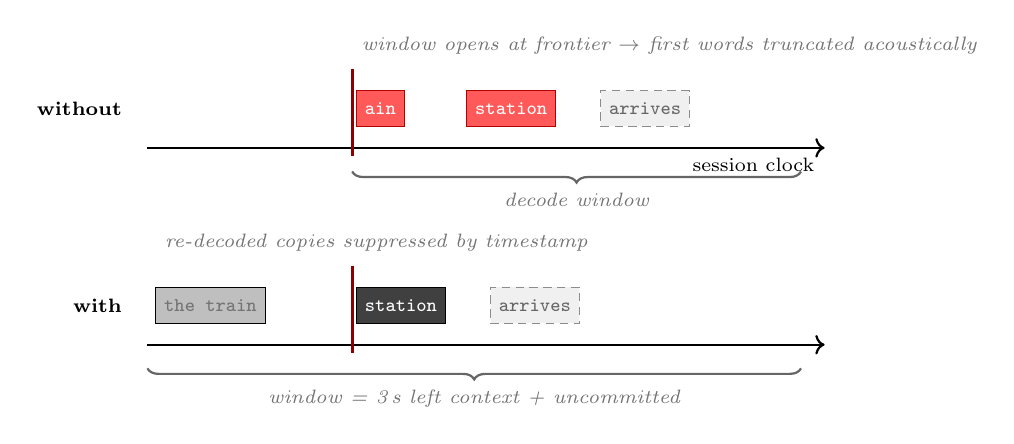
\begin{tikzpicture}[x=1cm]
  \panelrow{without}
  \draw[axis, ->] (0,-0.25) -- (8.6,-0.25) node[lbl, below left] {session clock};
  \draw[frontier] (2.6,-0.35) -- (2.6,0.75);
  \node[bad]  at (2.65,0.25) {ain};
  \node[bad, anchor=west] at (4.05,0.25) {station};
  \node[tentative, anchor=west] at (5.75,0.25) {arrives};
  \node[note] at (2.6,1.05) {window opens at frontier $\rightarrow$ first words truncated acoustically};
  \draw[win] (2.6,-0.55) -- (8.3,-0.55) node[midway, below=4pt, note, anchor=north] {decode window};
  \begin{scope}[yshift=-2.5cm]
  \panelrow{with}
  \draw[axis, ->] (0,-0.25) -- (8.6,-0.25);
  \draw[frontier] (2.6,-0.35) -- (2.6,0.75);
  \node[word, fill=black!25, text=black!55] at (0.1,0.25) {the train};
  \node[note] at (0.1,1.05) {re-decoded copies suppressed by timestamp};
  \node[committed] at (2.65,0.25) {station};
  \node[tentative, anchor=west] at (4.35,0.25) {arrives};
  \draw[win] (0.0,-0.55) -- (8.3,-0.55) node[midway, below=4pt, note, anchor=north]
    {window = 3\,s left context + uncommitted};
  \end{scope}
\end{tikzpicture}
\end{center}

\section*{2. \texttt{frame\_tolerance\_s = 0.02} --- one decoder frame of drift}

\textbf{Without:} a re-decode re-times the last committed word's end 15\,ms past
the frontier; it survives the boundary filter and commits \emph{again} ---
append-only means the duplicate is permanent and invisible to the retraction
reducer. \textbf{With:} anything ending within one Whisper frame (20\,ms) of the
frontier is treated as re-decoded committed audio.

\begin{center}
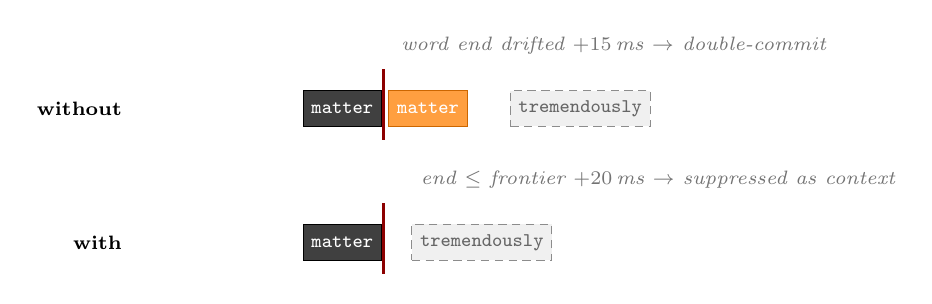
\begin{tikzpicture}[x=1cm]
  \panelrow{without}
  \draw[frontier] (3.0,-0.15) -- (3.0,0.75);
  \node[committed, anchor=east] at (2.98,0.25) {matter};
  \node[dup] at (3.06,0.25) {matter};
  \node[tentative, anchor=west] at (4.6,0.25) {tremendously};
  \node[note] at (3.1,1.05) {word end drifted $+15$\,ms $\rightarrow$ double-commit};
  \begin{scope}[yshift=-1.7cm]
  \panelrow{with}
  \draw[frontier] (3.0,-0.15) -- (3.0,0.75);
  \node[committed, anchor=east] at (2.98,0.25) {matter};
  \node[tentative] at (3.35,0.25) {tremendously};
  \node[note] at (3.35,1.05) {end $\le$ frontier $+20$\,ms $\rightarrow$ suppressed as context};
  \end{scope}
\end{tikzpicture}
\end{center}

\section*{3. \texttt{edge\_guard\_s = 0.6} --- agreement is not enough at the edge}

\textbf{Without:} a word cut off at the buffer edge makes the model hallucinate
a completion --- \emph{the same completion, with good probability, two ticks in
a row}. Agreement commits it; the real word later differs. \textbf{With:} words
ending in the last 600\,ms can never commit, agreed or not. This is the
structural defense (C7.4): distance from the edge, not confidence, is the test.

\begin{center}
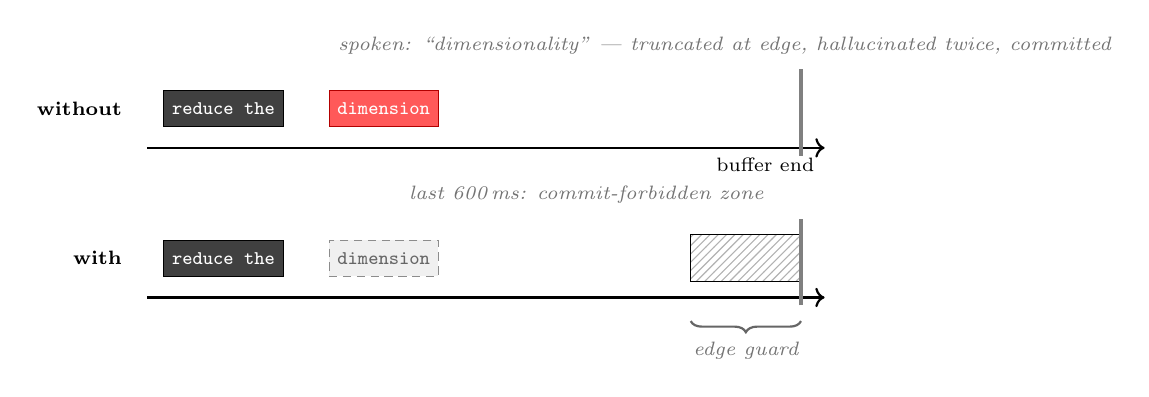
\begin{tikzpicture}[x=1cm]
  \panelrow{without}
  \draw[axis, ->] (0,-0.25) -- (8.6,-0.25) node[lbl, below left] {buffer end};
  \node[committed] at (0.2,0.25) {reduce the};
  \node[bad, anchor=west] at (2.3,0.25) {dimension};
  \node[note] at (2.3,1.05) {spoken: ``dimensionality'' --- truncated at edge, hallucinated twice, committed};
  \draw[frontier, black!50] (8.3,-0.35) -- (8.3,0.75);
  \begin{scope}[yshift=-1.9cm]
  \panelrow{with}
  \draw[axis, ->] (0,-0.25) -- (8.6,-0.25);
  \node[committed] at (0.2,0.25) {reduce the};
  \node[tentative, anchor=west] at (2.3,0.25) {dimension};
  \draw[pattern=north east lines, pattern color=black!30] (6.9,-0.05) rectangle (8.3,0.55);
  \node[note] at (3.2,1.05) {last 600\,ms: commit-forbidden zone};
  \draw[frontier, black!50] (8.3,-0.35) -- (8.3,0.75);
  \draw[win] (6.9,-0.55) -- (8.3,-0.55) node[midway, below=4pt, note, anchor=north] {edge guard};
  \end{scope}
\end{tikzpicture}
\end{center}

\section*{4. \texttt{word\_prob\_floor = 0.5} --- a veto, not a rejection}

\textbf{Without:} an agreed word at 0.31 probability commits permanently.
\textbf{With:} the commit scan stops at the first agreed word under the floor;
the word stays tentative and re-tries next tick with more audio behind it.
Vetoes only withhold --- they never edit --- so the retraction guarantee holds.

\emph{Field note (2026-08-05 trace diagnosis):} the floor's own failure mode is
\textbf{hostage-taking} --- on utterance 16 of the gate fixture, one word at
$p \approx 0.3$ held a nine-word agreed prefix behind it for three consecutive
ticks, until the holdback valve (\S6) burst-committed all ten unverified. One
low word can convert a healthy agreement run into a forced commit; the
per-tick stall counters (\S6) now make this visible per session.

\begin{center}
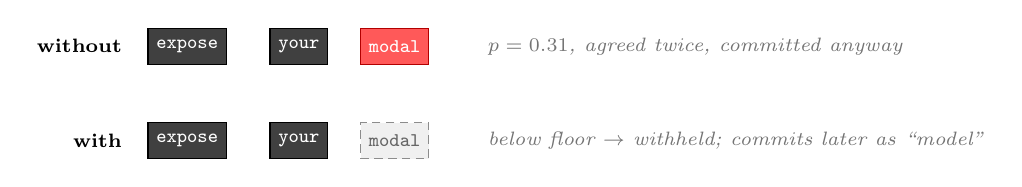
\begin{tikzpicture}[x=1cm]
  \panelrow{without}
  \node[committed] at (0,0.25) {expose};
  \node[committed, anchor=west] at (1.55,0.25) {your};
  \node[bad, anchor=west] at (2.7,0.25) {modal};
  \node[note, anchor=west] at (4.2,0.25) {$p=0.31$, agreed twice, committed anyway};
  \begin{scope}[yshift=-1.2cm]
  \panelrow{with}
  \node[committed] at (0,0.25) {expose};
  \node[committed, anchor=west] at (1.55,0.25) {your};
  \node[tentative, anchor=west] at (2.7,0.25) {modal};
  \node[note, anchor=west] at (4.2,0.25) {below floor $\rightarrow$ withheld; commits later as ``model''};
  \end{scope}
\end{tikzpicture}
\end{center}

\section*{5. The terminal-word rule (structural --- no knob)}

The last word of a hypothesis never commits: Whisper re-punctuates and
re-capitalizes it on nearly every pass, and committed text takes the surface
form of the \emph{newer} hypothesis. Field note (2026-08-04 wire log): this is
exactly why sentence-final punctuation drops when a commit boundary lands on a
sentence end --- the period existed only while the word was terminal.

\emph{Measured and settled (2026-08-05, offline replay on the gate fixture):}
committing the \emph{older} surface instead was evaluated against the one-shot
reference --- 18 divergent commits, prev-correct 11 vs prev-spurious 6. Both
hypotheses fabricate punctuation in both directions, and the same word commits
\emph{with} its period when the cut lands after the sentence boundary: the
defect is cut-position-dependent, not hypothesis-choice-dependent. Current
behavior stands; a punctuation-aware hybrid is parked for v4.2.

\begin{center}
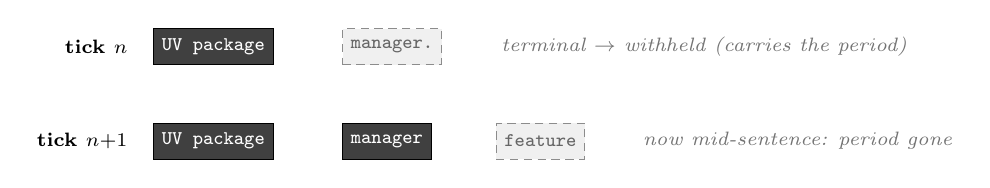
\begin{tikzpicture}[x=1cm]
  \panelrow{tick $n$}
  \node[committed] at (0,0.25) {UV package};
  \node[tentative, anchor=west] at (2.4,0.25) {manager.};
  \node[note, anchor=west] at (4.3,0.25) {terminal $\rightarrow$ withheld (carries the period)};
  \begin{scope}[yshift=-1.2cm]
  \panelrow{tick $n{+}1$}
  \node[committed] at (0,0.25) {UV package};
  \node[committed, anchor=west] at (2.4,0.25) {manager};
  \node[tentative, anchor=west] at (4.35,0.25) {feature};
  \node[note, anchor=west] at (6.1,0.25) {now mid-sentence: period gone};
  \end{scope}
\end{tikzpicture}
\end{center}

\section*{6. \texttt{max\_holdback\_ticks = 6} --- the anti-stall valve}

\textbf{Without:} disfluent speech makes consecutive hypotheses flip-flop; the
agreed prefix stops growing and the frontier stalls \emph{forever} --- unbounded
commit lag. \textbf{With:} after 6 stalled ticks ($6\times750\,\mathrm{ms} =
4.5$\,s) the newest hypothesis force-commits without agreement or the
probability floor --- but never past the edge guard. The valve's ledger from the
2026-08-04/05 field runs (impromptu speech, clean measurement):
\texttt{force\_commit\_rate} 8.7\% --- how often it fired;
\texttt{forced\_span\_wer} 14.3\% --- the quality price of committing unagreed
text; \texttt{commit\_lag\_max} 4.1--6.1\,s --- the bound at work. The
stall-reason counters (C9.3, landed 2026-08-05) decompose \emph{why} the valve
gets armed: of 96 zero-commit ticks on the gate fixture, 55 were the terminal
guard (agreement reaching only the last word), 20 the probability floor, 18
genuine divergence, 3 the edge guard. The v4.2 tuning question is therefore
short-agreement behavior --- not generic hypothesis churn.

\begin{center}
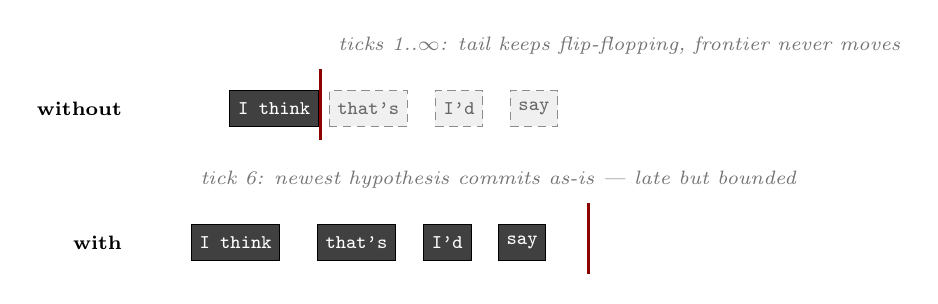
\begin{tikzpicture}[x=1cm]
  \panelrow{without}
  \draw[frontier] (2.2,-0.15) -- (2.2,0.75);
  \node[committed, anchor=east] at (2.18,0.25) {I think};
  \node[tentative] at (2.3,0.25) {that's};
  \node[tentative, anchor=west] at (3.65,0.25) {I'd};
  \node[tentative, anchor=west] at (4.6,0.25) {say};
  \node[note] at (2.3,1.05) {ticks 1..$\infty$: tail keeps flip-flopping, frontier never moves};
  \begin{scope}[yshift=-1.7cm]
  \panelrow{with}
  \draw[frontier] (5.6,-0.15) -- (5.6,0.75);
  \node[committed] at (0.55,0.25) {I think};
  \node[committed, anchor=west] at (2.15,0.25) {that's};
  \node[committed, anchor=west] at (3.5,0.25) {I'd};
  \node[committed, anchor=west] at (4.45,0.25) {say};
  \node[note] at (0.55,1.05) {tick 6: newest hypothesis commits as-is --- late but bounded};
  \end{scope}
\end{tikzpicture}
\end{center}

\section*{7. \texttt{max\_uncommitted\_s = 24} + \texttt{safety\_s = 3} --- the 30\,s wall}

Whisper's input is a fixed 30\,s window; \texttt{pad\_or\_trim} \emph{silently
truncates} anything longer. The invariant $3 + 24 + 3 = 30$ (enforced in
\texttt{validate()}) makes silent truncation impossible. \textbf{Without:} the
uncommitted span grows past the wall and the model simply never hears the
overflow --- unaccounted audio loss. \textbf{With:} \texttt{plan\_window}
reports the overflow and the session drops the \emph{oldest} uncommitted
samples explicitly, counted in \texttt{dropped\_audio\_ms}. The 2026-08-04 u3
run slid three 79\,s utterances through this and reported \texttt{dropped\_audio\_ms
= 0} with zero retractions --- the slide worked without ever needing the drop.

\begin{center}
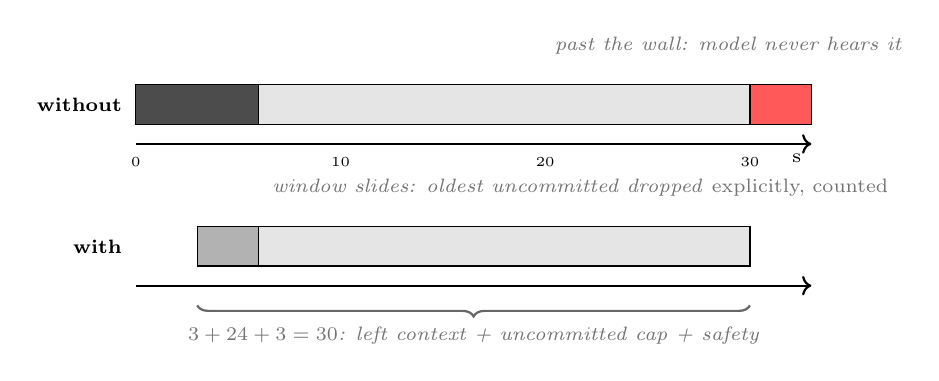
\begin{tikzpicture}[x=0.26cm]
  \panelrow{without}
  \draw[axis, ->] (0,-0.25) -- (33,-0.25) node[lbl, below left] {s};
  \foreach \x in {0,10,20,30} \node[lbl, below, font=\tiny] at (\x,-0.3) {\x};
  \draw[fill=black!70] (0,0) rectangle (6,0.5);
  \draw[fill=black!10] (6,0) rectangle (30,0.5);
  \draw[fill=red!65] (30,0) rectangle (33,0.5);
  \node[note] at (20,1.0) {past the wall: model never hears it};
  \begin{scope}[yshift=-1.8cm]
  \panelrow{with}
  \draw[axis, ->] (0,-0.25) -- (33,-0.25);
  \draw[fill=black!30] (3,0) rectangle (6,0.5);
  \draw[fill=black!10] (6,0) rectangle (30,0.5);
  \node[note] at (6.2,1.0) {window slides: oldest uncommitted dropped \emph{explicitly, counted}};
  \draw[win] (3,-0.5) -- (30,-0.5) node[midway, below=4pt, note, anchor=north]
    {$3 + 24 + 3 = 30$: left context + uncommitted cap + safety};
  \end{scope}
\end{tikzpicture}
\end{center}

\section*{8. \texttt{flush\_left\_context\_s = 1.0} --- context priced in latency}

The flush decode (end of utterance --- silence is ground truth, commit
everything) opens only 1\,s before the frontier, not 3: the flush sits on the
finalization-latency path, and \emph{every second of context here is paid
directly in the user-visible finalization number} (gate: $\le 0.5$\,s after the
first utterance; 2026-08-04 measured 0.544\,s). \texttt{validate()} refuses a
flush context larger than \texttt{left\_context\_s} --- retention only
guarantees that much audio still exists.

\section*{9. The twin residue guards --- \texttt{seam\_tolerance\_s = 0.10} (C7.12) and \texttt{tick\_residue\_tolerance\_s = 0.20} (C7.13)}

Same disease, two symptoms. The frontier is a DTW word-end \emph{estimate} that
lands tens of ms early, so acoustic residue of the last committed word leaks
into the next decode and re-emits (``very Very'', 2026-08-02 field finding).
Both guards are conjunctions on the \emph{leading} word matching the last
committed word --- but they gate on opposite ends, because the impostors differ:

\begin{center}
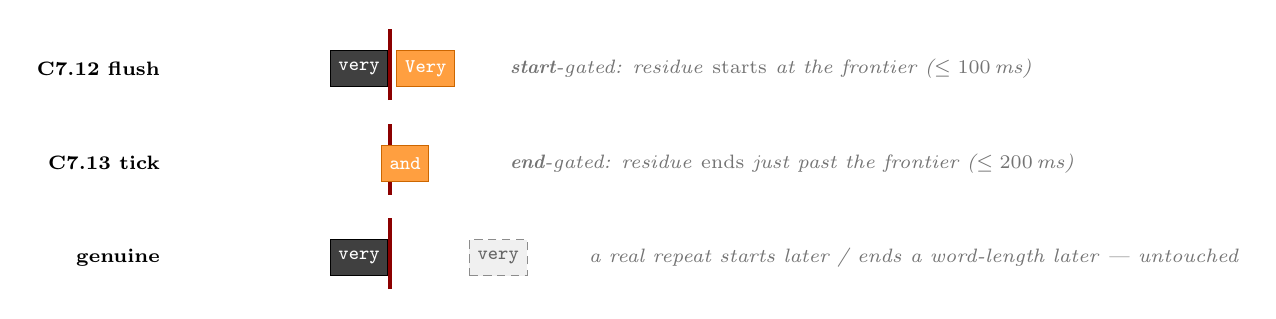
\begin{tikzpicture}[x=1cm]
  \panelrow{C7.12 flush}
  \draw[frontier] (2.6,-0.15) -- (2.6,0.75);
  \node[committed, anchor=east] at (2.58,0.25) {very};
  \node[dup] at (2.68,0.25) {Very};
  \node[note, anchor=west] at (4.0,0.25)
    {\textbf{start}-gated: residue \emph{starts} at the frontier ($\le 100$\,ms)};
  \begin{scope}[yshift=-1.2cm]
  \panelrow{C7.13 tick}
  \draw[frontier] (2.6,-0.15) -- (2.6,0.75);
  \node[dup, anchor=east] at (3.1,0.25) {and};
  \node[note, anchor=west] at (4.0,0.25)
    {\textbf{end}-gated: residue \emph{ends} just past the frontier ($\le 200$\,ms)};
  \end{scope}
  \begin{scope}[yshift=-2.4cm]
  \panelrow{genuine}
  \draw[frontier] (2.6,-0.15) -- (2.6,0.75);
  \node[committed, anchor=east] at (2.58,0.25) {very};
  \node[tentative] at (3.6,0.25) {very};
  \node[note, anchor=west] at (5.0,0.25)
    {a real repeat starts later / ends a word-length later --- untouched};
  \end{scope}
\end{tikzpicture}
\end{center}

Accepted residual risk, stated in the code: a genuine immediate repeat falling
inside the tolerance is indistinguishable by any local rule and is dropped ---
so every suppression is counted on the session-close log line, keeping the
trade observable. 2026-08-04 field ledger: 3 seam catches, 2--14 tick-residue
suppressions per session, zero visible duplicates.

\section*{10. \texttt{merge\_glued\_words} --- the decoder-edge merge (C7.14, new)}

Runs \emph{before} everything above, at the decoder edge. faster-whisper marks
word-initial tokens with a leading space and emits glued continuations
(\texttt{"-fold"}, \texttt{"\%"}) without one. The policy previously stripped
that signal and re-joined committed words with plain spaces --- fabricating
\texttt{"K -fold"} and \texttt{"95 \%"} (9 artifact tokens per 412 words live,
each scoring $\approx$2 WER errors against the space-preserving one-shot
reference). The merge makes each glued cluster \emph{one} Word, so a commit
boundary can never split it and every downstream space-join is correct by
construction.

\begin{center}
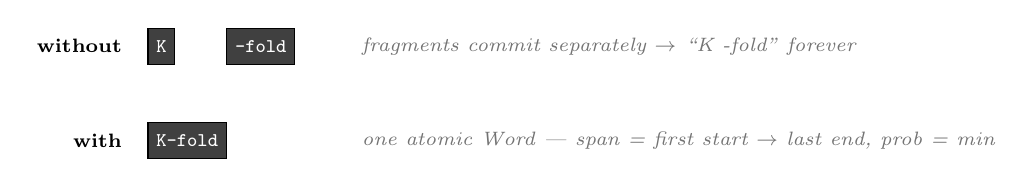
\begin{tikzpicture}[x=1cm]
  \panelrow{without}
  \node[committed] at (0,0.25) {K};
  \node[committed, anchor=west] at (1.0,0.25) {-fold};
  \node[note, anchor=west] at (2.6,0.25)
    {fragments commit separately $\rightarrow$ ``K -fold'' forever};
  \begin{scope}[yshift=-1.2cm]
  \panelrow{with}
  \node[committed] at (0,0.25) {K-fold};
  \node[note, anchor=west] at (2.6,0.25)
    {one atomic Word --- span = first start $\rightarrow$ last end, prob = min};
  \end{scope}
\end{tikzpicture}
\end{center}

Measured effect on the gate fixture: \texttt{wer\_micro} 4.55\% $\rightarrow$
3.68\% --- that share of the ``streaming quality gap'' was an assembly
artifact, not recognition.

\section*{Coda --- how the knobs met the field on 2026-08-04/05}

One recording of disfluent, self-correcting impromptu speech exercised every
mechanism above: the holdback valve fired at 8.7\% (its ledger, \S6), the slide
handled $3\times79$\,s utterances without dropping a sample (\S7), the twin
guards caught frontier residue while one burst-commit landed past the C7.12
start-gate (\S9's accepted residual, now diagnosed --- see \S4's hostage note),
the terminal-word rule explained the missing sentence periods (\S5, measured
and settled), and the flush context closed to 13\,ms over its latency gate
(\S8) once the decoder-edge merge (\S10) cleaned the measurement. Every number
above is now reproducible offline: the C9.3 trace + \texttt{policy\_replay.py}
re-ran 291 live GPU ticks with zero drift. Tuning any one knob moves a number
you can now name --- and test in milliseconds.

\end{document}
